\documentclass[12pt]{article}
\usepackage{amsmath, amssymb, amsthm}
\usepackage{graphicx}
\usepackage{float}
\usepackage[margin=1in]{geometry}
\usepackage{hyperref}
\usepackage{booktabs}

\title{EECE5644 Fall 2025 - Assignment 1}
\author{Steven Chen}
\date{October 16 2025}

\begin{document}

\maketitle

\section*{Abstract}
This report presents the implementation and analysis of three classification approaches on a 3-dimensional dataset with two classes. The methods include: (1) Optimal ERM classification with known true distributions, (2) Naive Bayes classification with model mismatch, and (3) Fisher Linear Discriminant Analysis. Performance is evaluated using ROC curves and probability of error metrics.

\section*{Code Repository}
The complete MATLAB code for this assignment is available at: \\
\url{https://github.com/GuestAGuy/EECE5644}

% \tableofcontents

\newpage

% =============================================================================
% QUESTION 1
% =============================================================================

\section{Question 1: Classification of 3D Gaussian Data}

The probability density function for a 3-dimensional real-valued random vector $\mathbf{X}$ is given by:
\[
p(\mathbf{x}) = p(\mathbf{x}|L=0)P(L=0) + p(\mathbf{x}|L=1)P(L=1)
\]
where $L$ is the true class label with priors $P(L=0)=0.65$ and $P(L=1)=0.35$.

The class-conditional PDFs are:
\begin{align*}
p(\mathbf{x}|L=0) &= \mathcal{N}(\mathbf{x}|\mathbf{m}_{0},\mathbf{C}_{0}) \\
p(\mathbf{x}|L=1) &= \mathcal{N}(\mathbf{x}|\mathbf{m}_{1},\mathbf{C}_{1})
\end{align*}

With parameters:
\[
\mathbf{m}_{0} = \begin{bmatrix} -1/2 \\ -1/2 \\ -1/2 \end{bmatrix}, \quad
\mathbf{C}_{0} = \begin{bmatrix} 1 & -0.5 & 0.3 \\ -0.5 & 1 & -0.5 \\ 0.3 & -0.5 & 1 \end{bmatrix}
\]
\[
\mathbf{m}_{1} = \begin{bmatrix} 1 \\ 1 \\ 1 \end{bmatrix}, \quad
\mathbf{C}_{1} = \begin{bmatrix} 1 & 0.3 & -0.2 \\ 0.3 & 1 & 0.3 \\ -0.2 & 0.3 & 1 \end{bmatrix}
\]

A dataset of 10,000 samples was generated from this distribution for analysis.
\begin{figure}[H]
    \centering
    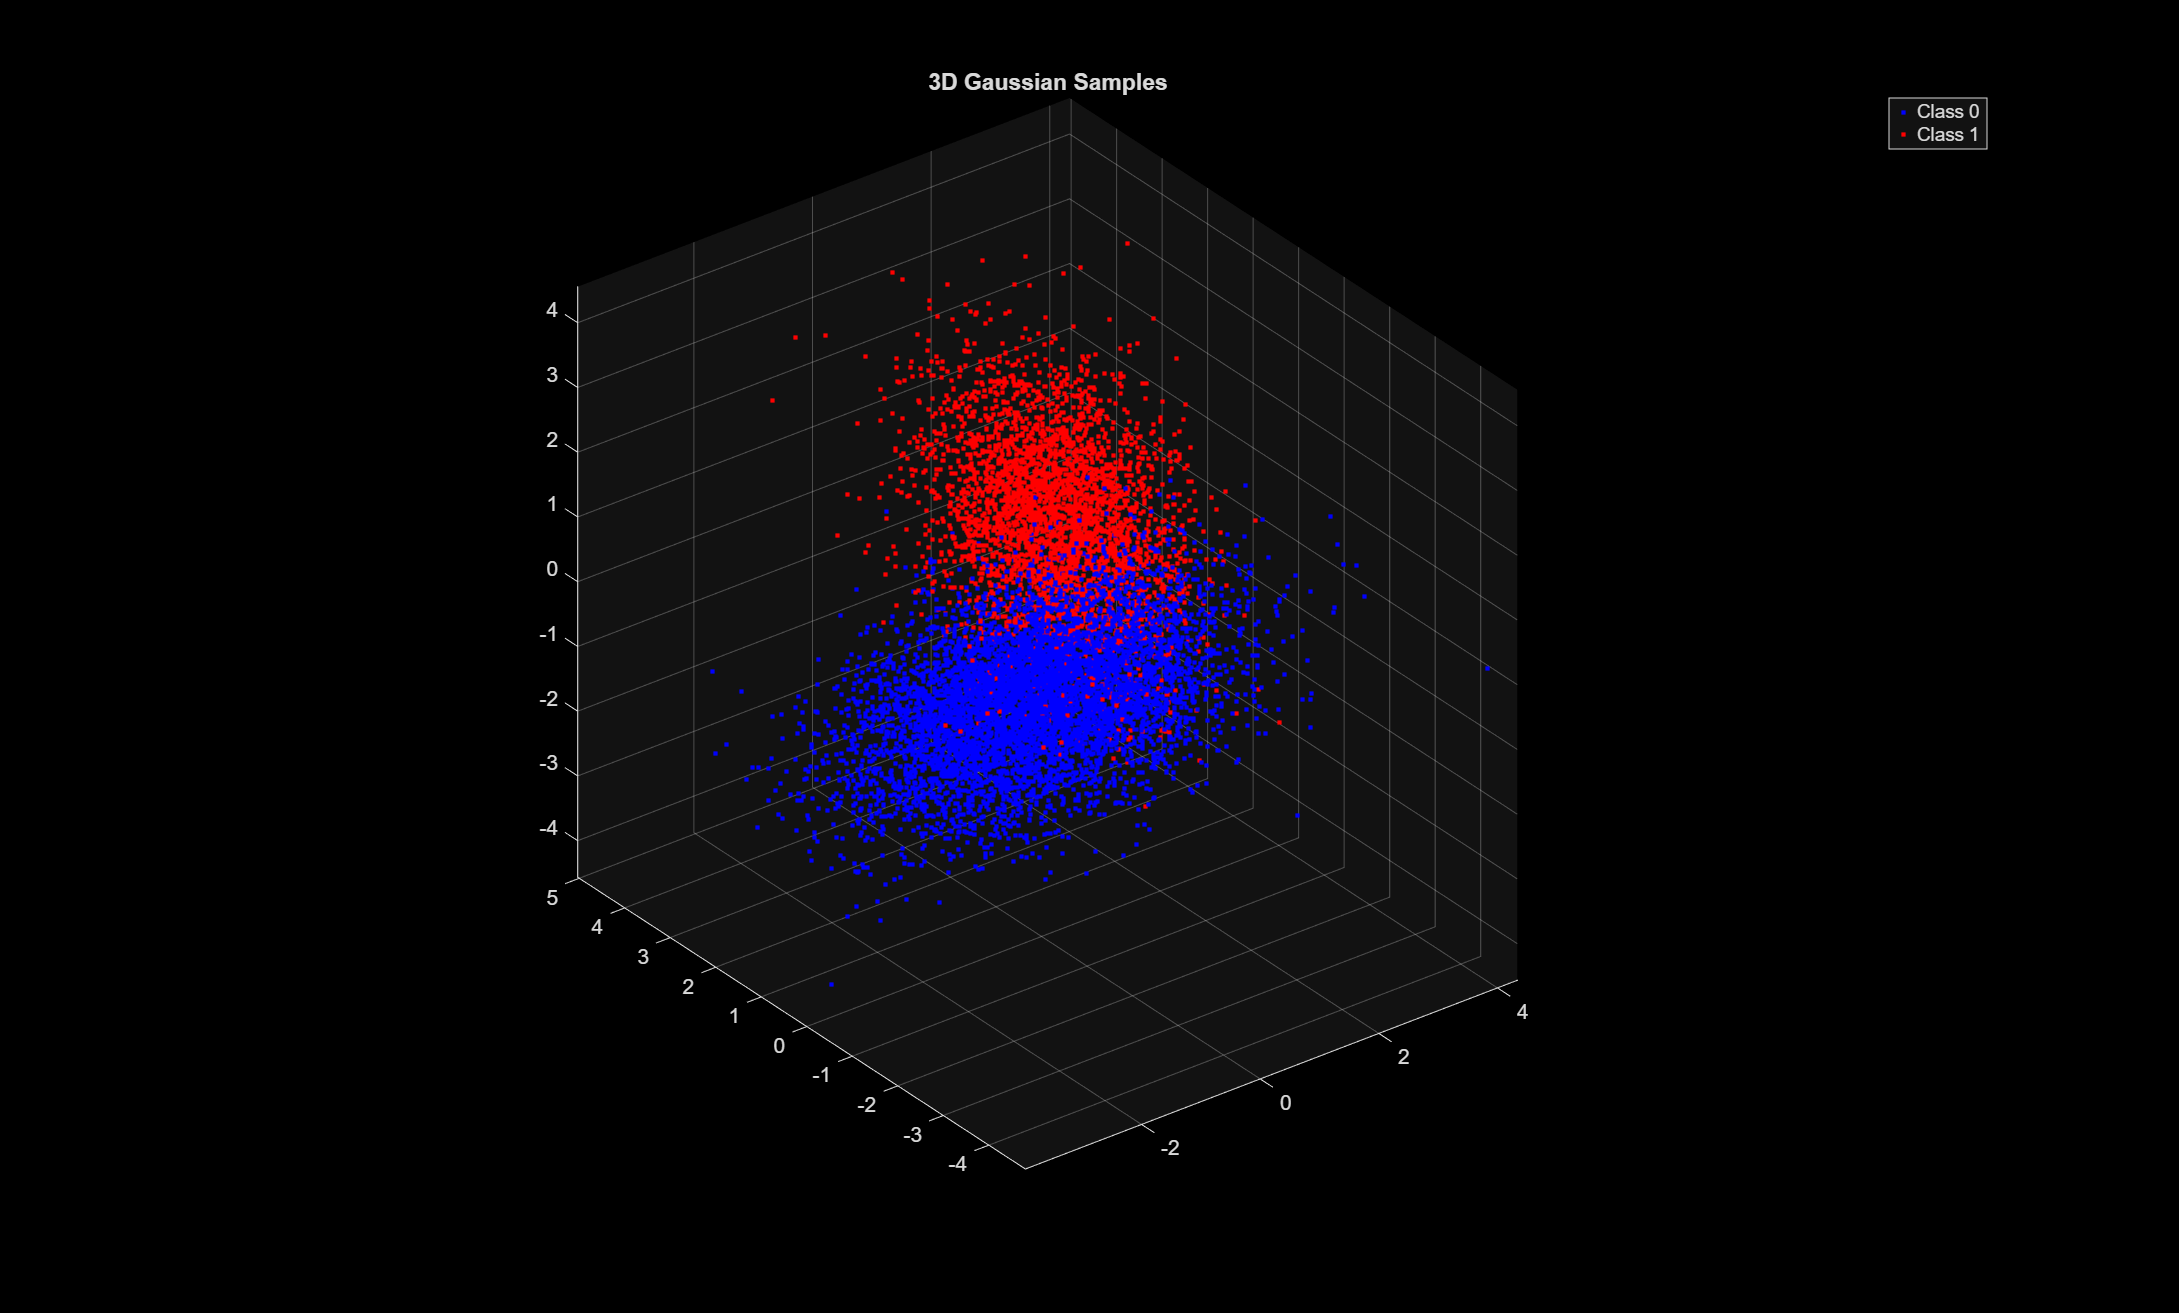
\includegraphics[width=0.8\textwidth]{gaussian_classes.png}
    \label{fig:gaussian_classes}
\end{figure}



\newpage

% =============================================================================
% PART A - ERM CLASSIFICATION
% =============================================================================
%In Part A, we're building the theoretically optimal classifier by using the exact known data distributions. We calculate how likely each sample is from each class, then use a likelihood ratio test with different thresholds to trace out an ROC curve. We find the threshold that gives the fewest mistakes, mark that point on the ROC curve, and compare our practical results with the theoretical optimum.
\subsection{Part A: ERM Classification with True Data Distribution}

\subsubsection{Theoretical setup}

The minimum expected risk classification rule is derived under the 0-1 loss function, where incorrect decisions are penalized equally and correct decisions incur no cost. This loss structure is defined as:

\begin{equation}
\lambda_{dl} = \begin{cases} 
0 & \text{if } d = l \quad \text{(correct decision)} \\
1 & \text{if } d \neq l \quad \text{(incorrect decision)}
\end{cases}
\end{equation}

For this binary classification problem, the expected risk conditioned on observation $\mathbf{x}$ is expressed as:

\begin{equation}
R(D=d|\mathbf{x}) = \sum_{l=0}^{1} \lambda_{dl} P(L=l|\mathbf{x})
\end{equation}

The optimal decision rule minimizes this conditional risk, leading to the maximum a posteriori (MAP) classification rule:

\begin{equation}
\delta^*(\mathbf{x}) = \arg\max_{j \in \{0,1\}} P(L=j|\mathbf{x})
\end{equation}

Through application of Bayes' theorem, this MAP rule simplifies to a likelihood ratio test:

\begin{equation}
\frac{p(\mathbf{x}|L=1)}{p(\mathbf{x}|L=0)} \stackrel{D=1}{\underset{D=0}{\gtrless}} \gamma
\end{equation}

The theoretical threshold for minimum probability of error is derived from the class priors and loss values:

\begin{equation}
\gamma = \frac{(\lambda_{10} - \lambda_{00})}{(\lambda_{01} - \lambda_{11})} \cdot \frac{P(L=0)}{P(L=1)} = \frac{0.65}{0.35} \approx 1.8571
\end{equation}

The class-conditional probability density functions are multivariate Gaussians, specified by:

\begin{align*}
p(\mathbf{x}|L=0) &= \frac{1}{(2\pi)^{3/2}|\mathbf{C}_0|^{1/2}} \exp\left(-\frac{1}{2}(\mathbf{x}-\mathbf{m}_0)^T\mathbf{C}_0^{-1}(\mathbf{x}-\mathbf{m}_0)\right) \\
p(\mathbf{x}|L=1) &= \frac{1}{(2\pi)^{3/2}|\mathbf{C}_1|^{1/2}} \exp\left(-\frac{1}{2}(\mathbf{x}-\mathbf{m}_1)^T\mathbf{C}_1^{-1}(\mathbf{x}-\mathbf{m}_1)\right)
\end{align*}


\subsubsection{Implementation and Results}
\href{https://github.com/GuestAGuy/EECE5644/blob/main/HW1Q1/HW1Q1.m}{https://github.com/GuestAGuy/EECE5644/blob/main/HW1Q1/HW1Q1.m}
By calculating likelihood ratios for all 10,000 samples and sweeping through threshold values from $10^{-3}$ to $10^{3}$ to generate the ROC curve.
\begin{figure}[H]
    \centering
    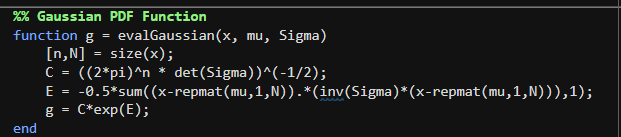
\includegraphics[width=0.7\linewidth]{matlab_eval_gaussian.png}
    \caption{Referenced code from "Code" folder "evalGaussian.m"}
\end{figure}

\begin{figure}[H]
    \centering
    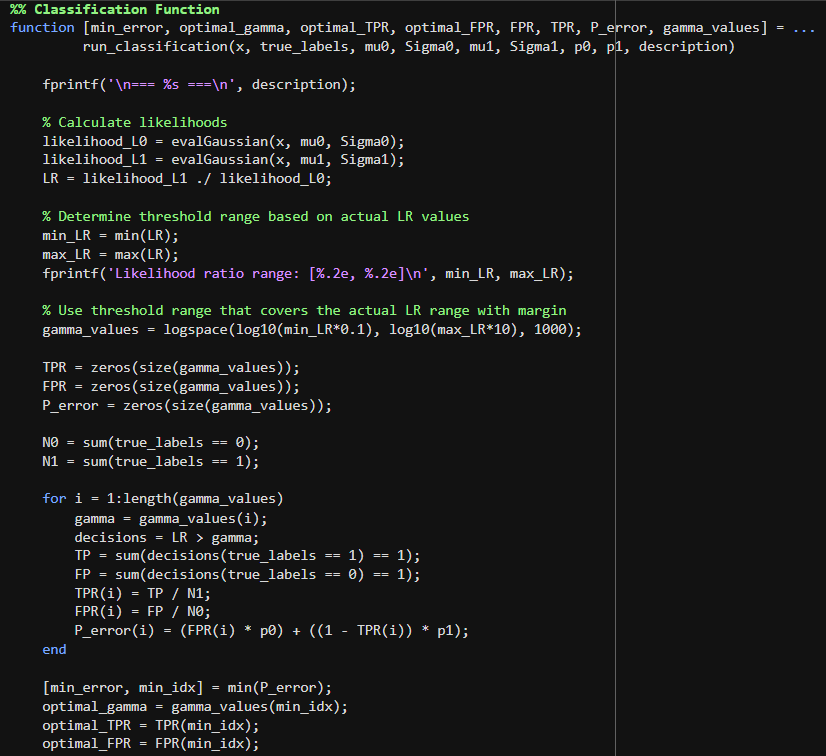
\includegraphics[width=0.9\linewidth]{matlab_classification_function.png}
    \caption{Matlab code Implementation for classification, it is written into function for reuse later in part b}
\end{figure}

Result from the code:
\begin{figure}[H]
    \centering
    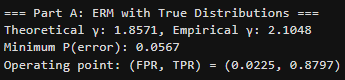
\includegraphics[width=0.5\linewidth]{resultA.png}
\end{figure}

\begin{figure}[H]
    \centering
    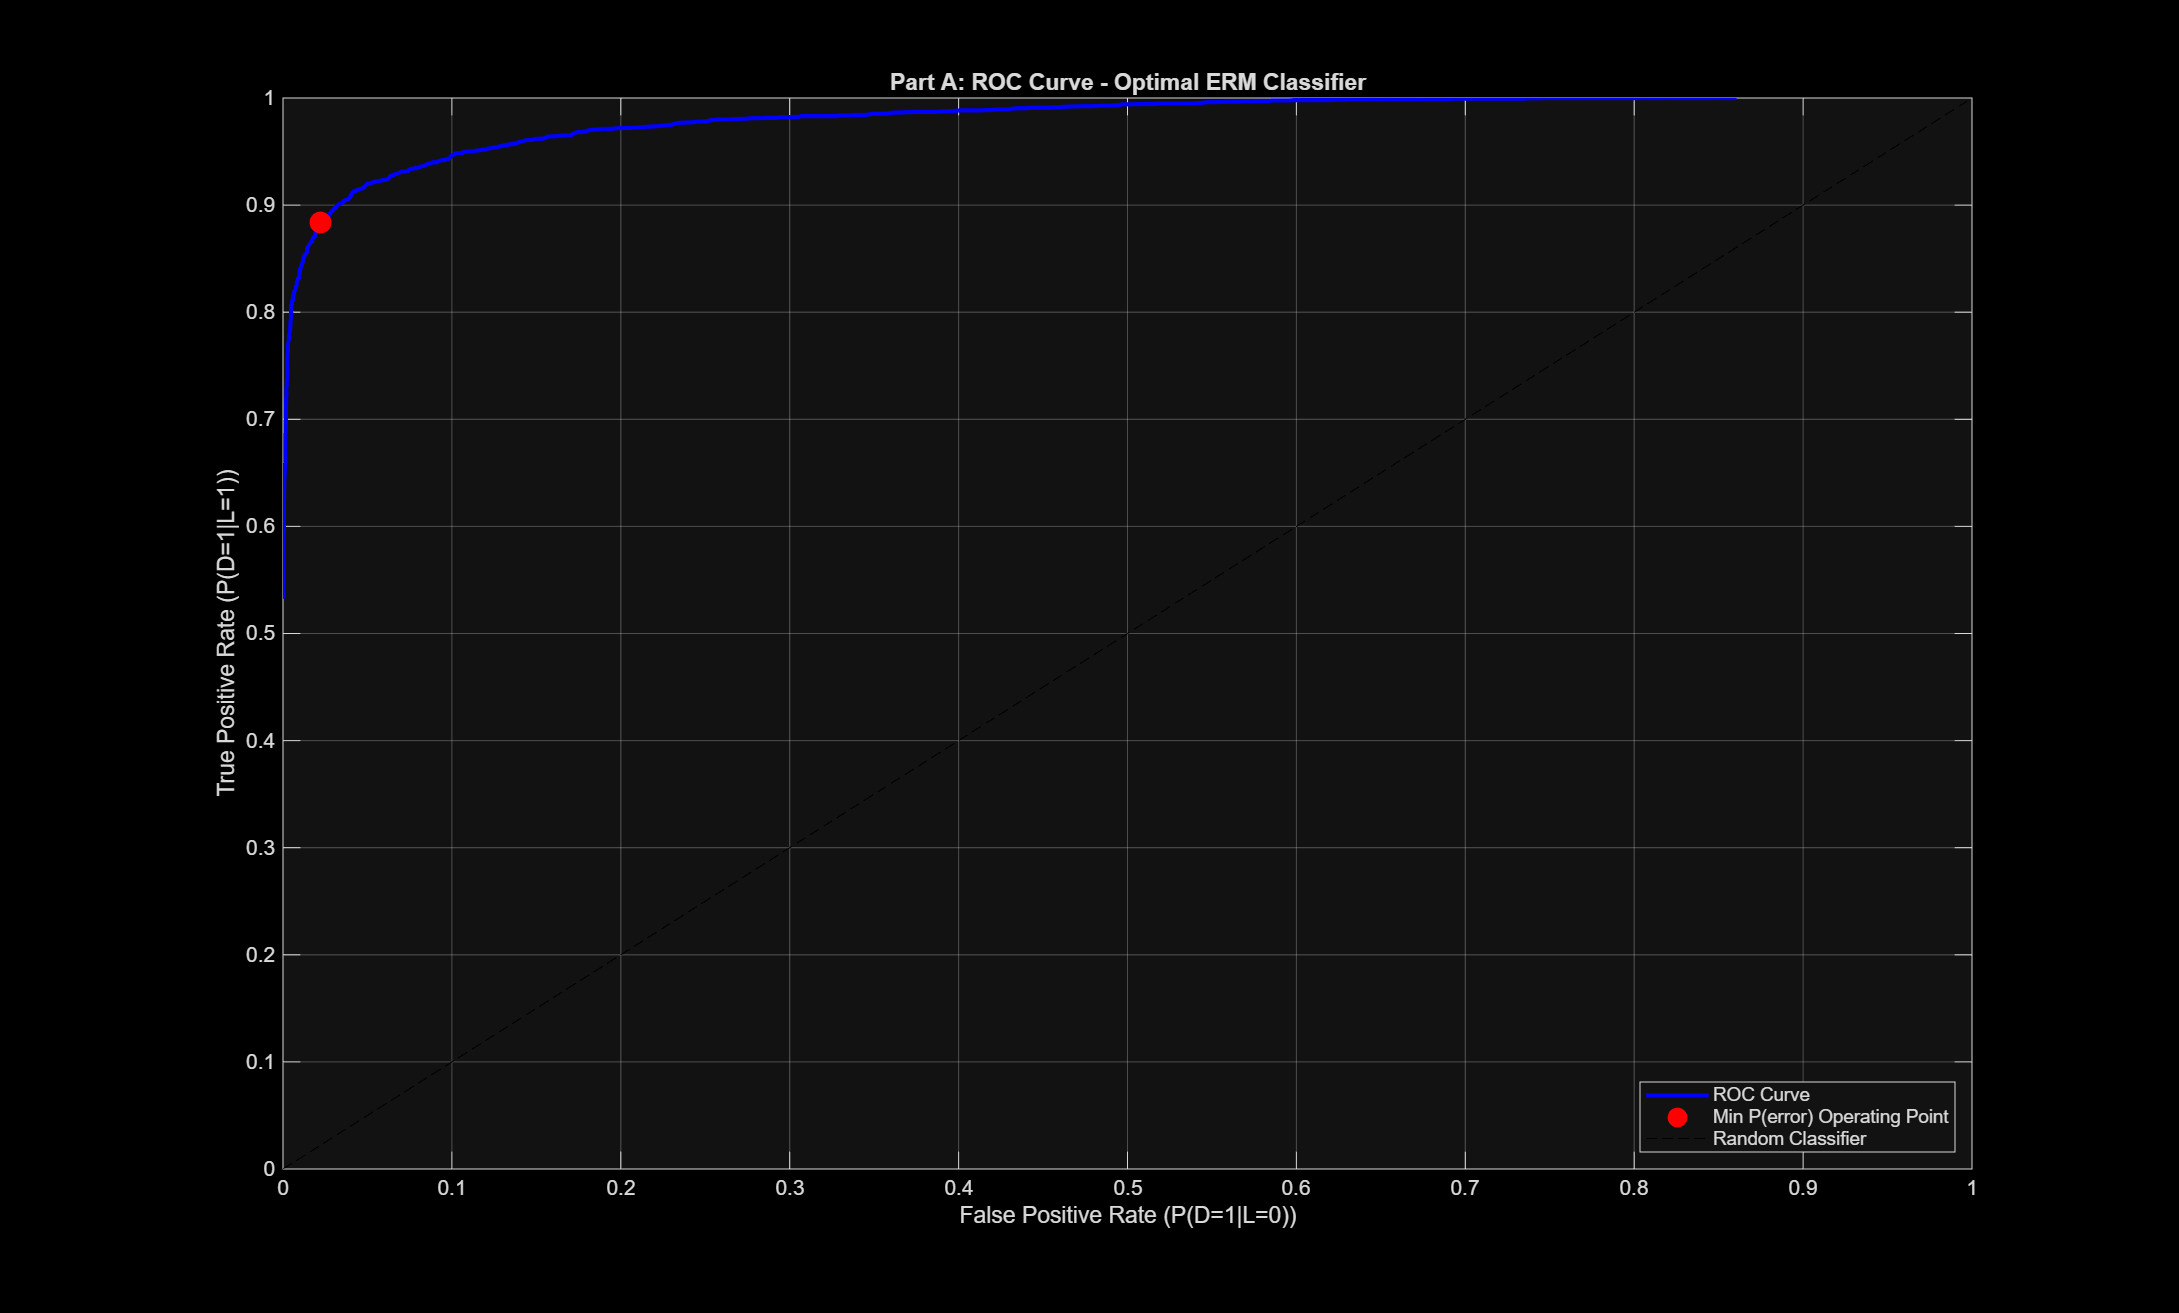
\includegraphics[width=0.8\textwidth]{partA_ROC.png}
\end{figure}

\subsubsection{Discussion}
Looking at the results, the empirical threshold we found 2.1048 is pretty close to the theoretical value of 1.8571. The small difference makes sense given we're working with a finite sample size of 10,000 - with infinite data, they should match exactly. The minimum error rate of about 5.67\% represents the best we can possibly do for this problem, which is actually pretty good! The ROC curve shows we can catch nearly 88\% of class 1 samples while only falsely alarming about 2.25\% of class 0 samples at the optimal point.

% =============================================================================
% PART B - NAIVE BAYES
% =============================================================================

\subsection{Part B: Naive Bayes Classification with Model Mismatch}
\subsubsection{Theoretical Framework}

In Part B, we analyze the impact of model mismatch by incorrectly assuming feature independence (Naive Bayes assumption). The likelihood ratio test structure remains:

\begin{equation}
\frac{p(\mathbf{x}|L=1)}{p(\mathbf{x}|L=0)} \stackrel{D=1}{\underset{D=0}{\gtrless}} \gamma
\end{equation}

With the same theoretical threshold (since priors and loss function are unchanged):
\begin{equation}
\gamma = \frac{P(L=0)}{P(L=1)} = \frac{0.65}{0.35} \approx 1.8571
\end{equation}

However, we now use incorrect class-conditional PDFs that assume identity covariance matrices:
\begin{align}
\mathbf{C}_0^{\text{naive}} = \mathbf{C}_1^{\text{naive}} = \mathbf{I} = \begin{bmatrix} 1 & 0 & 0 \\ 0 & 1 & 0 \\ 0 & 0 & 1 \end{bmatrix}
\end{align}


\subsubsection{Implementation and Results}

Implemented this by rewriting the same code from Part A into a function, but changing only the input covariance matrices to identity matrices. Everything else stayed the same.

\begin{figure}[H]
    \centering
    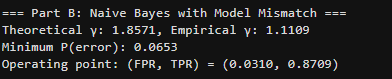
\includegraphics[width=0.5\linewidth]{resultB.png}
\end{figure}
\begin{figure}[H]
    \centering
    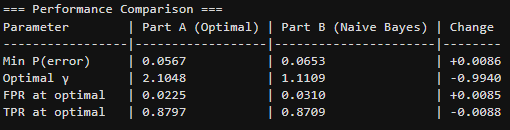
\includegraphics[width=0.65\linewidth]{AB_Comparison.png}
\end{figure}

\begin{figure}[H]
    \centering
    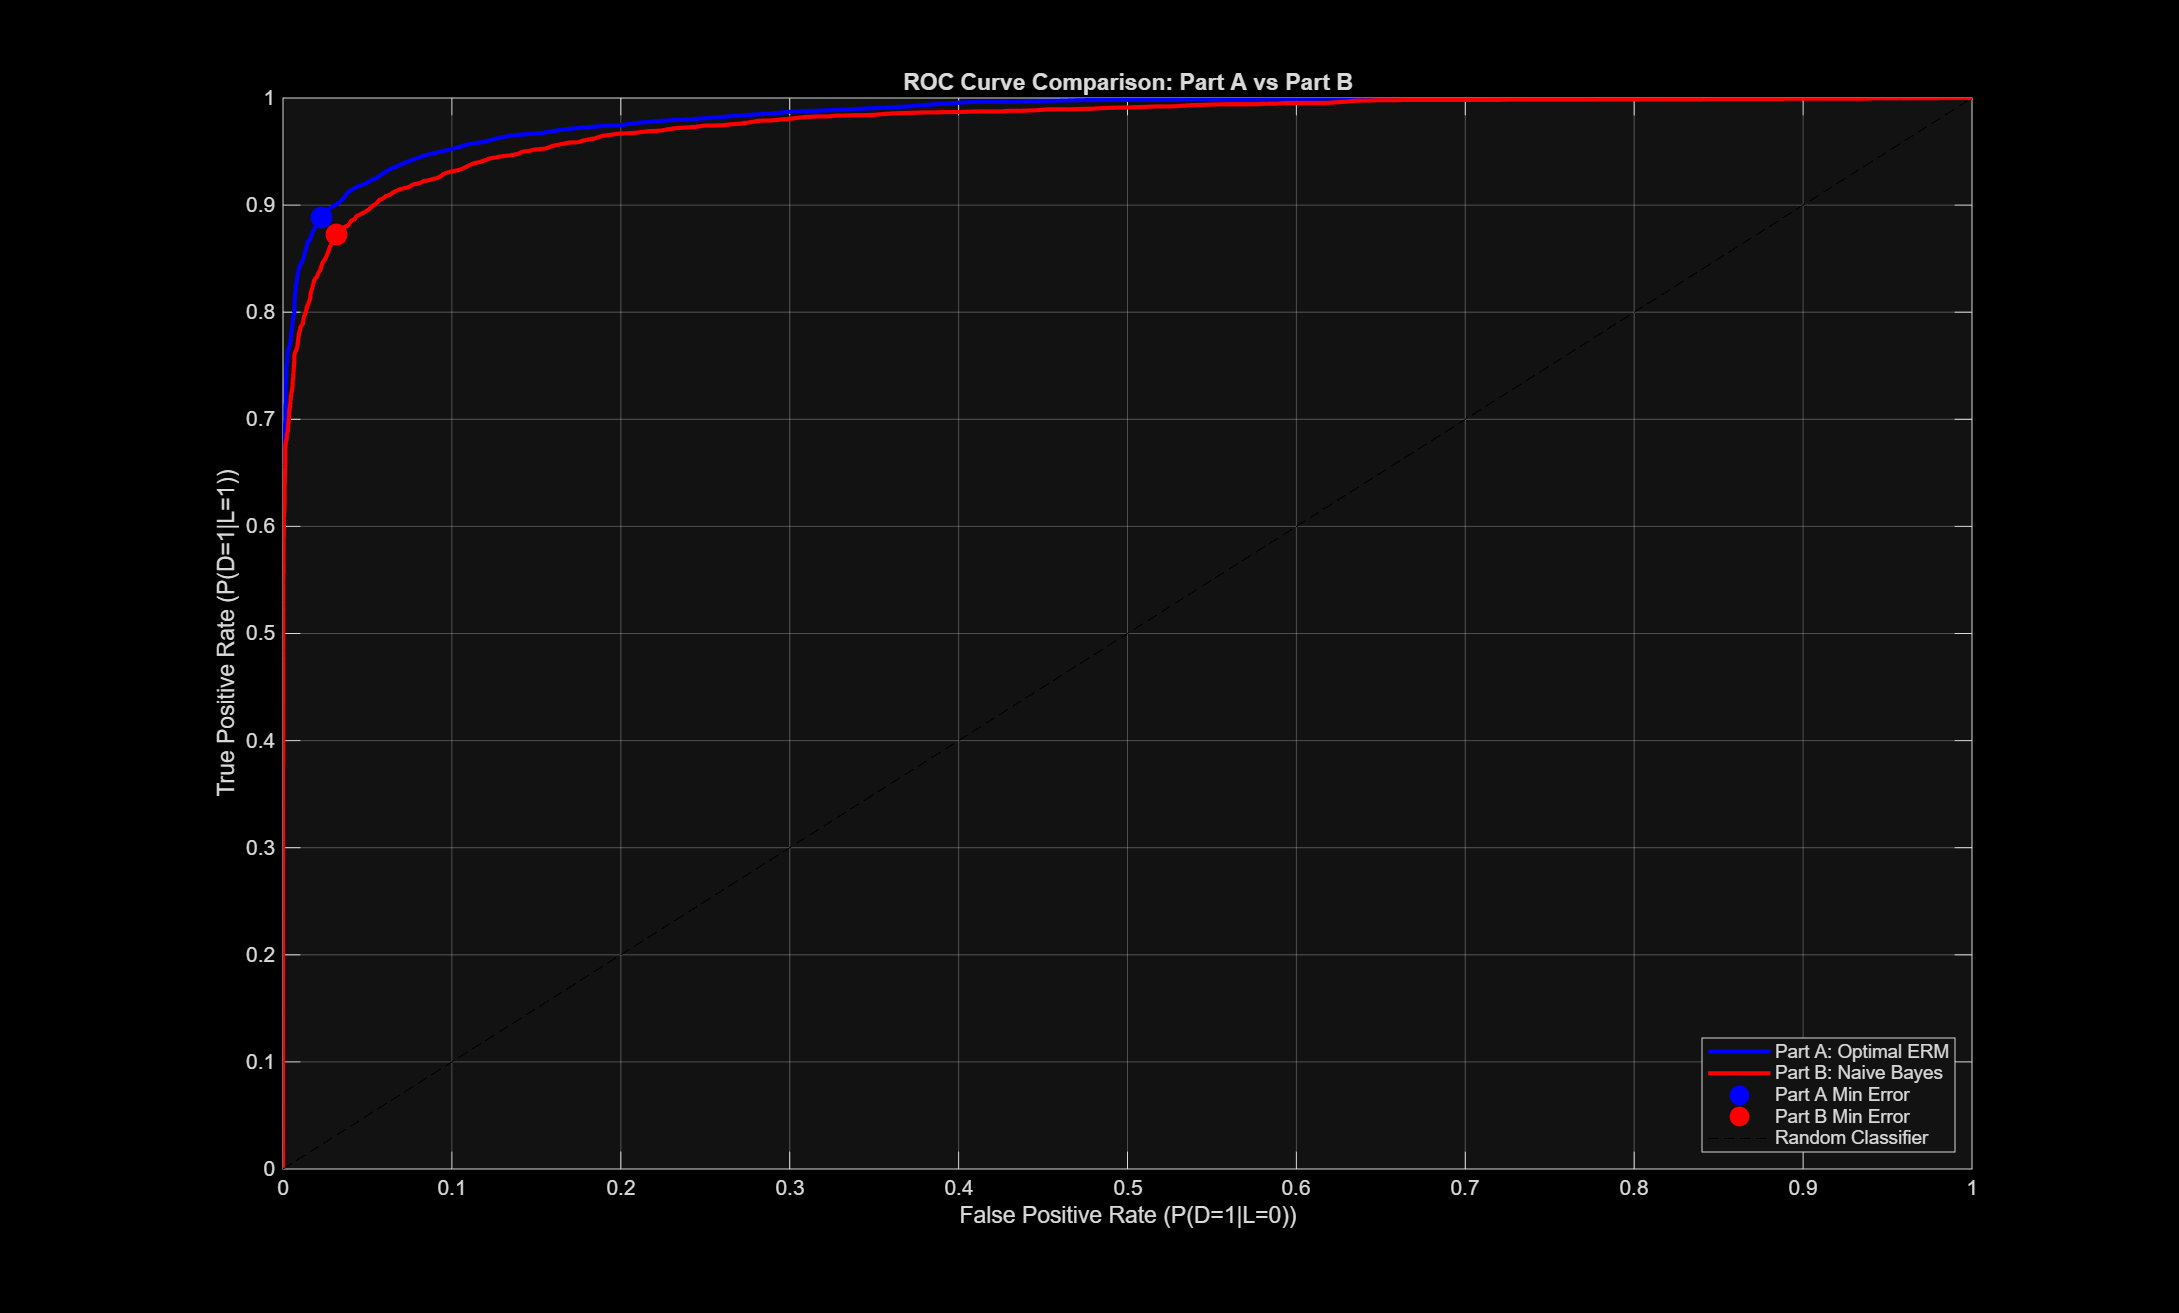
\includegraphics[width=0.7\textwidth]{partAB_ROC_comparison.png}
    \caption{ROC curve comparison showing how the Naive Bayes assumption degrades performance. The blue curve (Part A) is clearly better than the red curve (Part B).}
\end{figure}

\subsubsection{Discussion}
The model mismatch led to a clear performance drop - the error rate increased from 5.67\% to 6.53\%. The Naive Bayes classifier just doesn't separate the classes as well, catching about 87\% of class 1 samples but with more false alarms at 3.10\%. The optimal threshold also shifted quite a bit from 2.10 to 1.11, showing how the wrong model assumptions mess up the decision boundary. Basically, by assuming features are independent when they're actually correlated, we lose valuable information that could help tell the classes apart.
% =============================================================================
% PART C - FISHER LDA
% =============================================================================
\subsection{Part C: Fisher LDA Classification}

\subsubsection{Theoretical Framework}

Fisher LDA finds the optimal projection direction $\mathbf{w}$ that maximizes class separation. Following the derivation in the course notes, we define the between-class and within-class scatter matrices:

\[
\mathbf{S}_B = (\boldsymbol{\mu}_1 - \boldsymbol{\mu}_2)(\boldsymbol{\mu}_1 - \boldsymbol{\mu}_2)^T \quad \text{and} \quad \mathbf{S}_W = \boldsymbol{\Sigma}_1 + \boldsymbol{\Sigma}_2
\]

The objective is to maximize Fisher's criterion:
\[
J(\mathbf{w}) = \frac{\mathbf{w}^T \mathbf{S}_B \mathbf{w}}{\mathbf{w}^T \mathbf{S}_W \mathbf{w}}
\]

As derived in the notes, this leads to the generalized eigenvalue problem:
\[
\mathbf{S}_B \mathbf{w} = \lambda \mathbf{S}_W \mathbf{w}
\]

The solution is the eigenvector of $\mathbf{S}_W^{-1} \mathbf{S}_B$ corresponding to the largest eigenvalue, which gives us the optimal projection vector $\mathbf{w}_{LDA}$.

\subsubsection{Implementation and Results}

Implemented Fisher LDA by estimating the mean vectors and covariance matrices from our 10,000 samples, then solving the generalized eigenvalue problem to find the optimal projection direction.

\begin{figure}[H]
    \centering
    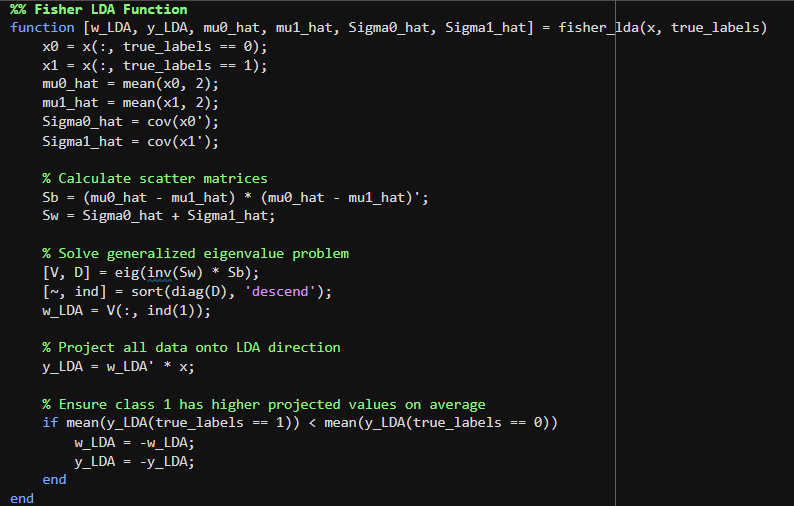
\includegraphics[width=0.65\linewidth]{matlab_FisherLDA.png}
    \caption{Referenced code from "Code" folder "fisherLDA.m"}
\end{figure}

\begin{figure}[H]
    \centering
    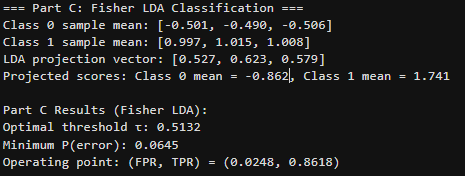
\includegraphics[width=0.6\linewidth]{resultC.png}
\end{figure}
\begin{figure}[H]
    \centering
    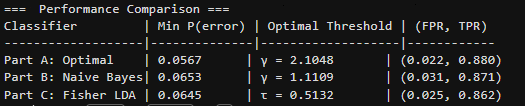
\includegraphics[width=0.6\linewidth]{PartsComparasion.png}
\end{figure}

\begin{figure}[H]
    \centering
    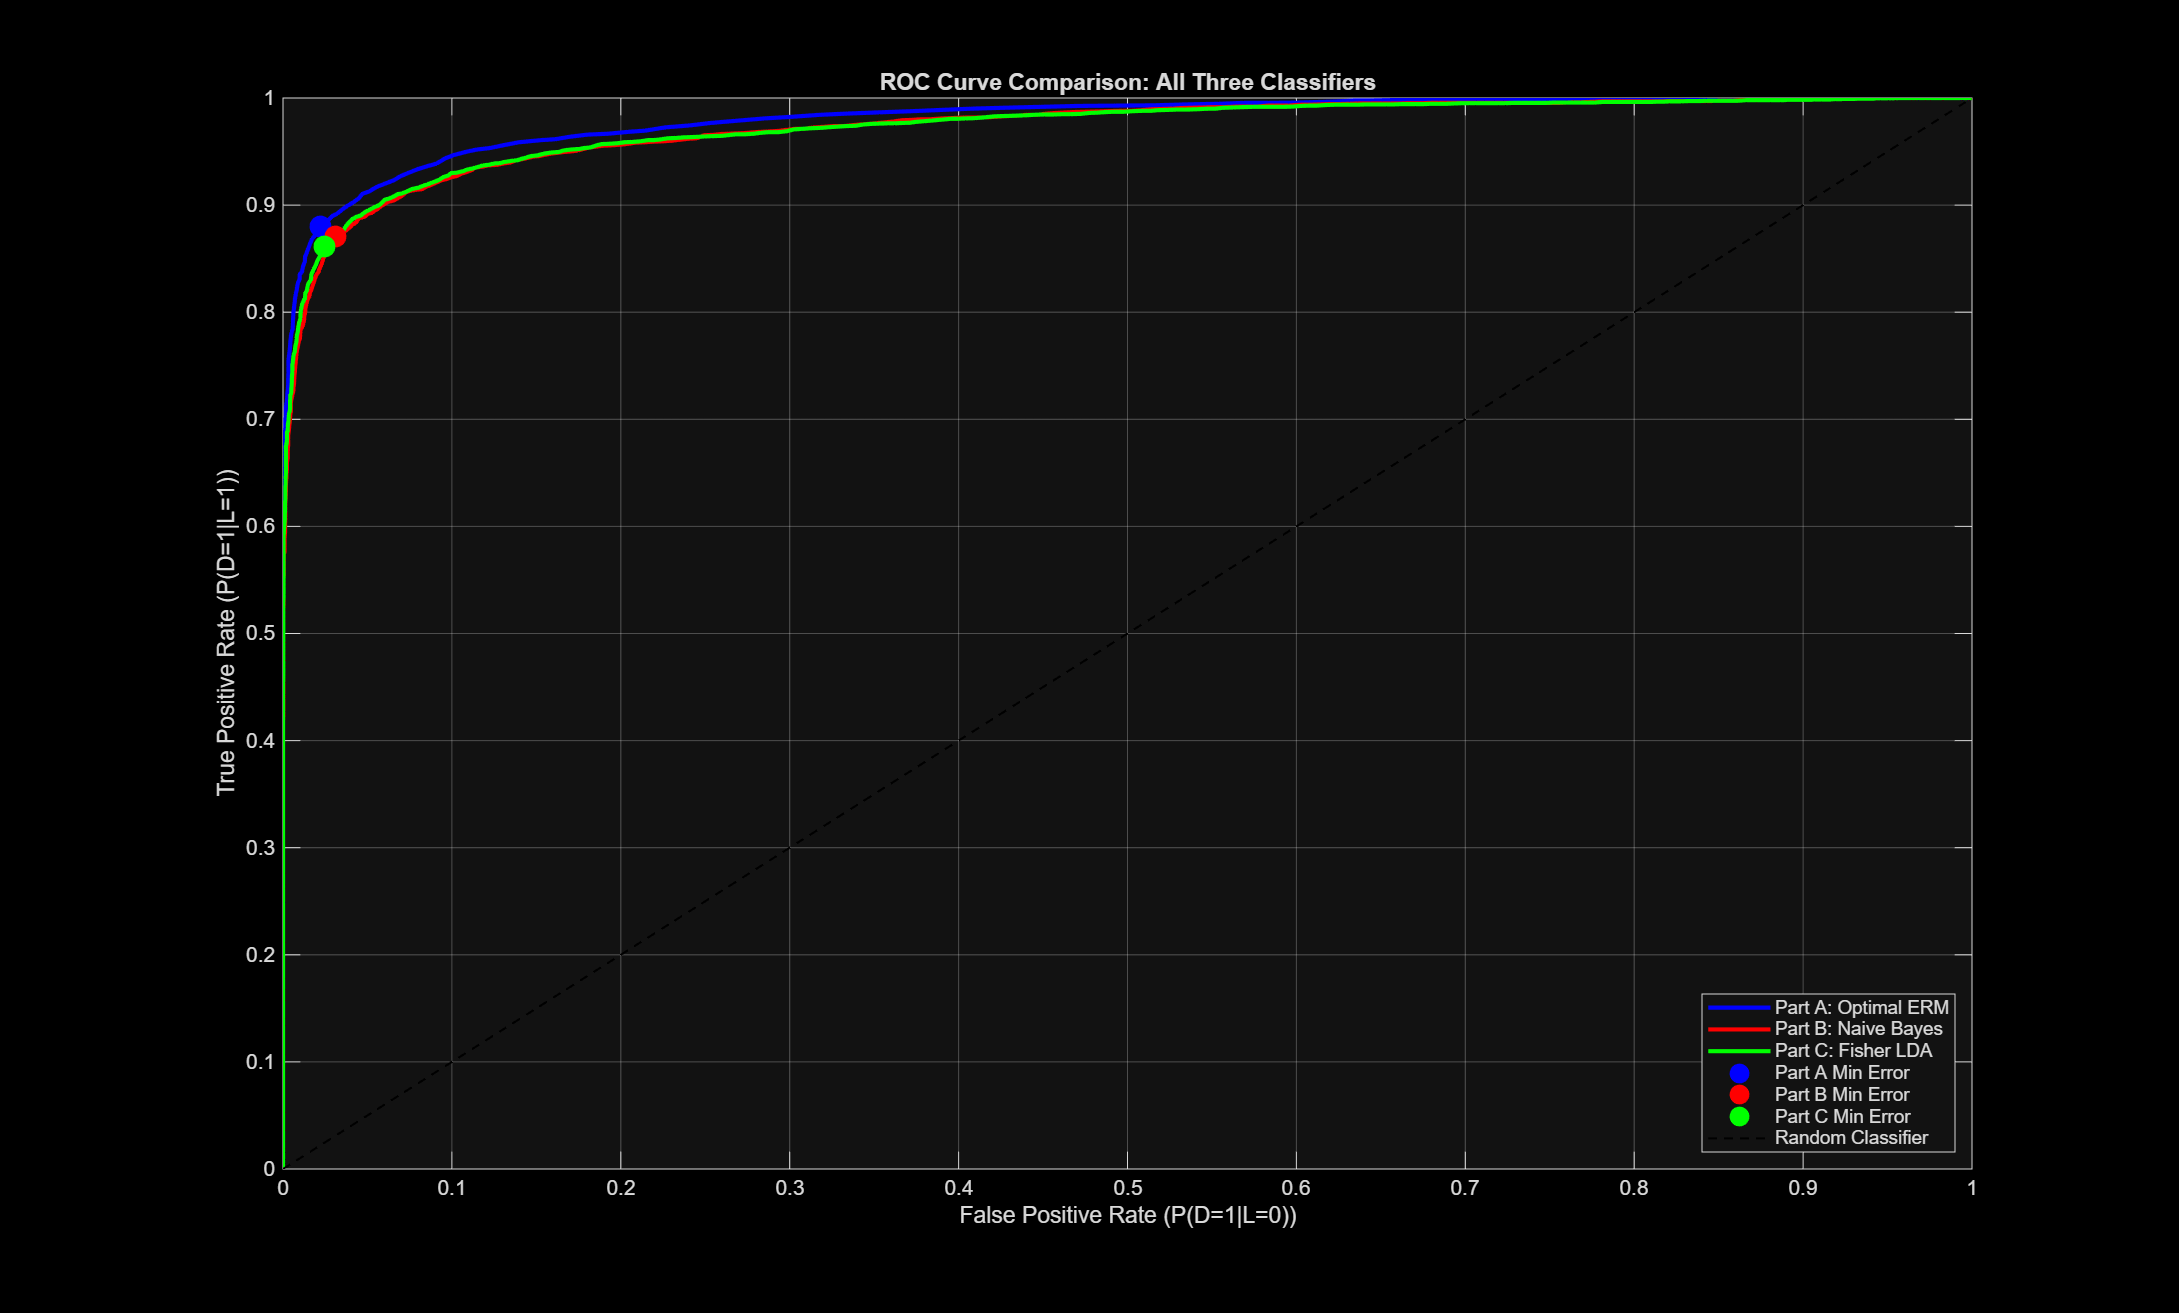
\includegraphics[width=0.8\textwidth]{partC_ROC_comparison_all.png}
    \caption{ROC curve comparison showing all three classifiers. Fisher LDA (green) performs between the optimal ERM and Naive Bayes approaches.}
\end{figure}

\begin{figure}[H]
    \centering
    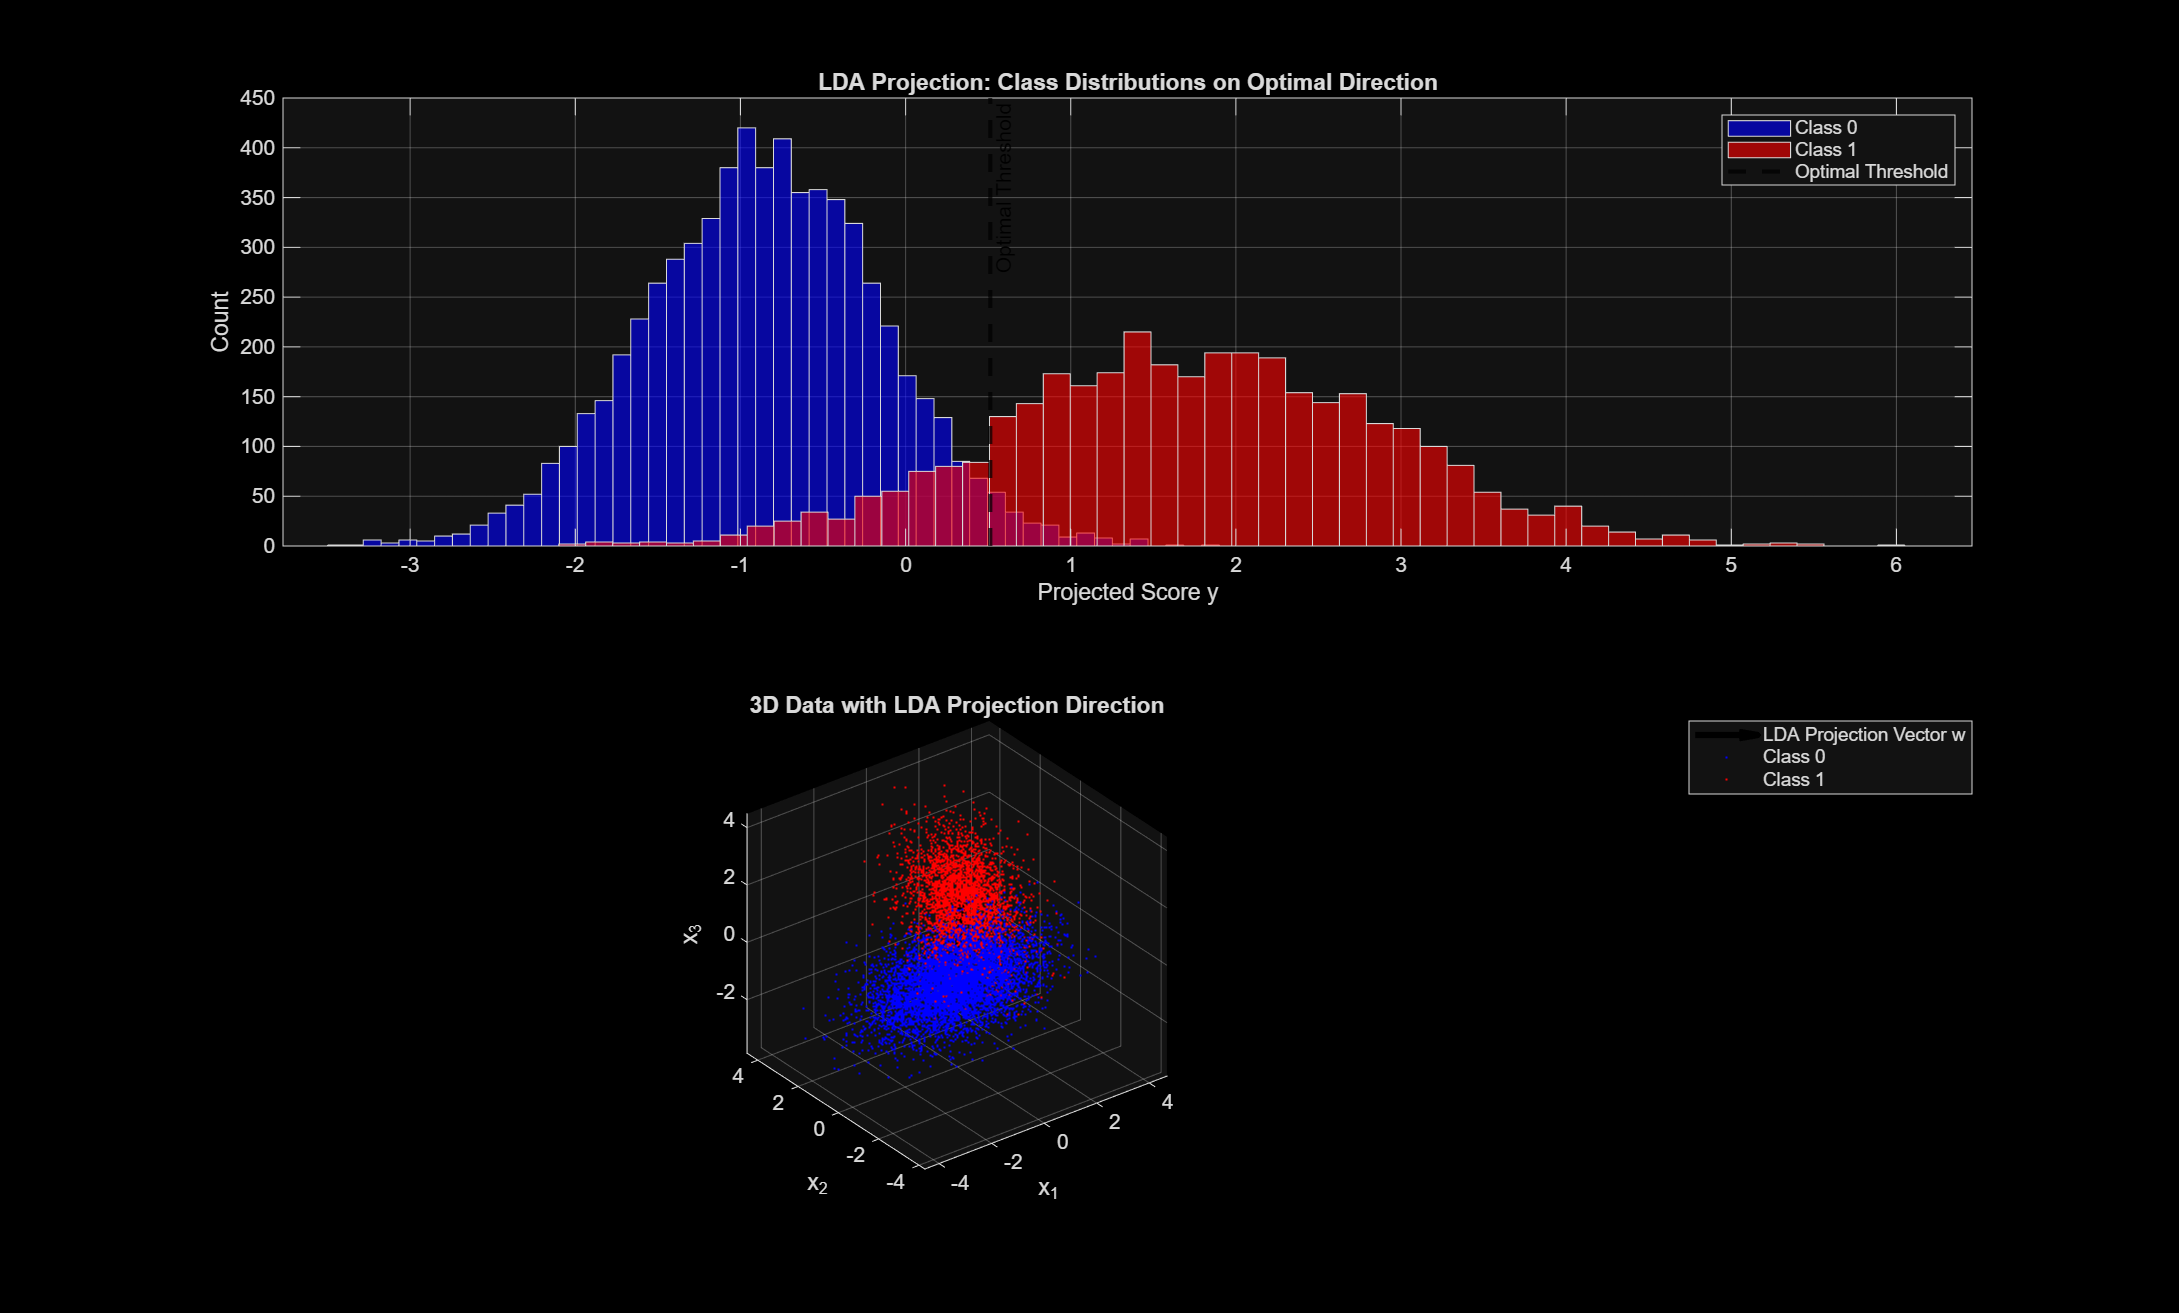
\includegraphics[width=0.8\textwidth]{partC_LDA_projection.png}
    \caption{LDA projection visualization. Top: Class distributions along the optimal projection direction. Bottom: 3D data with the LDA projection vector.}
\end{figure}

\subsubsection{Discussion}
Fisher LDA achieved a minimum probability of error of 6.45\%, performing between the optimal ERM classifier (5.67\%) and Naive Bayes (6.53\%). This aligns with theoretical expectations, as LDA finds the optimal linear separation while the true optimal boundary from Part A is quadratic due to differing covariance structures.

The LDA projection vector $\mathbf{w}_{LDA} = [0.527, 0.623, 0.579]^T$ effectively separates the classes, with projected means at -0.862 (class 0) and 1.741 (class 1). The optimal threshold $\tau = 0.5132$ achieves an operating point of (FPR, TPR) = (0.0248, 0.8618).

Compared to the previous classifiers, LDA demonstrates several key characteristics:
\begin{itemize}
\item \textbf{Vs. Optimal ERM}: LDA cannot achieve the optimal performance because it is constrained to linear decision boundaries, while the true optimal boundary is quadratic due to different covariance matrices
\item \textbf{Vs. Naive Bayes}: LDA outperforms Naive Bayes (6.45\% vs 6.53\% error) because it properly utilizes the estimated covariance structure rather than assuming feature independence
\item \textbf{Practical Value}: LDA provides a data-driven approach that estimates parameters from samples, making it applicable to real-world problems where true distributions are unknown
\end{itemize}

The estimated parameters closely approximate true distributions, demonstrating LDA's effectiveness as a practical balance between performance and real-world applicability when true distributions are unknown.
% =============================================================================
% QUESTION 2
% =============================================================================

\newpage
\section{Question 2: Classification with Gaussian Mixture Models}

\subsection{Problem Statement}
A 2-dimensional random vector $\mathbf{X}$ follows a mixture of four Gaussian distributions with equal priors $P(L=j) = 0.25$. The following Gaussian parameters were selected for this analysis:

\begin{align*}
\boldsymbol{\mu}_1 &= \begin{bmatrix} -1 \\ -1 \end{bmatrix}, \quad
\boldsymbol{\Sigma}_1 = \begin{bmatrix} 1 & 0.25 \\ 0.25 & 0.8 \end{bmatrix} \\
\boldsymbol{\mu}_2 &= \begin{bmatrix} 2 \\ -2 \end{bmatrix}, \quad
\boldsymbol{\Sigma}_2 = \begin{bmatrix} 0.8 & -0.5 \\ -0.5 & 1.2 \end{bmatrix} \\
\boldsymbol{\mu}_3 &= \begin{bmatrix} -3 \\ 1 \end{bmatrix}, \quad
\boldsymbol{\Sigma}_3 = \begin{bmatrix} 1.5 & 0.75 \\ 0.75 & 1 \end{bmatrix} \\
\boldsymbol{\mu}_4 &= \begin{bmatrix} 1.5 \\ 1.5 \end{bmatrix}, \quad
\boldsymbol{\Sigma}_4 = \begin{bmatrix} 2 & 0.7 \\ 0.7 & 1.5 \end{bmatrix}
\end{align*}

\subsection{Part A: MAP Classification with 0-1 Loss}

\subsubsection{Theoretical Framework}
For equal priors and 0-1 loss, the MAP decision rule simplifies to maximum likelihood:

\begin{equation}
\delta^*(\mathbf{x}) = \arg\max_{j \in \{1,2,3,4\}} p(\mathbf{x}|L=j)
\end{equation}

The Gaussian likelihood is computed using:
\begin{equation}
p(\mathbf{x}|L=j) = \frac{1}{2\pi|\boldsymbol{\Sigma}_j|^{1/2}} \exp\left(-\frac{1}{2}(\mathbf{x}-\boldsymbol{\mu}_j)^T\boldsymbol{\Sigma}_j^{-1}(\mathbf{x}-\boldsymbol{\mu}_j)\right)
\end{equation}

\subsubsection{Implementation}
The MAP classifier was implemented by computing Gaussian likelihoods for each class and selecting the maximum.


\href{https://github.com/GuestAGuy/EECE5644/blob/main/HW1Q2/HW1Q2.m}{https://github.com/GuestAGuy/EECE5644/blob/main/HW1Q2/HW1Q2.m}

\begin{figure}[H]
    \centering
    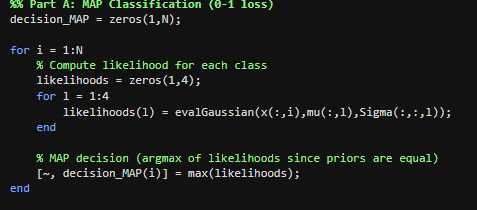
\includegraphics[width=0.6\textwidth]{q2_map_code.png}
    \caption{MAP classification implementation}
\end{figure}

\subsubsection{Results}

\begin{figure}[H]
    \centering
    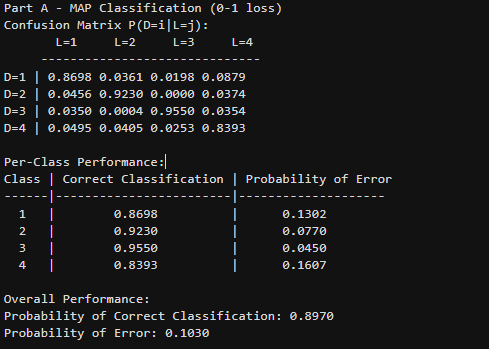
\includegraphics[width=0.5\textwidth]{q2_map_output.png}
\end{figure}

\begin{figure}[H]
    \centering
    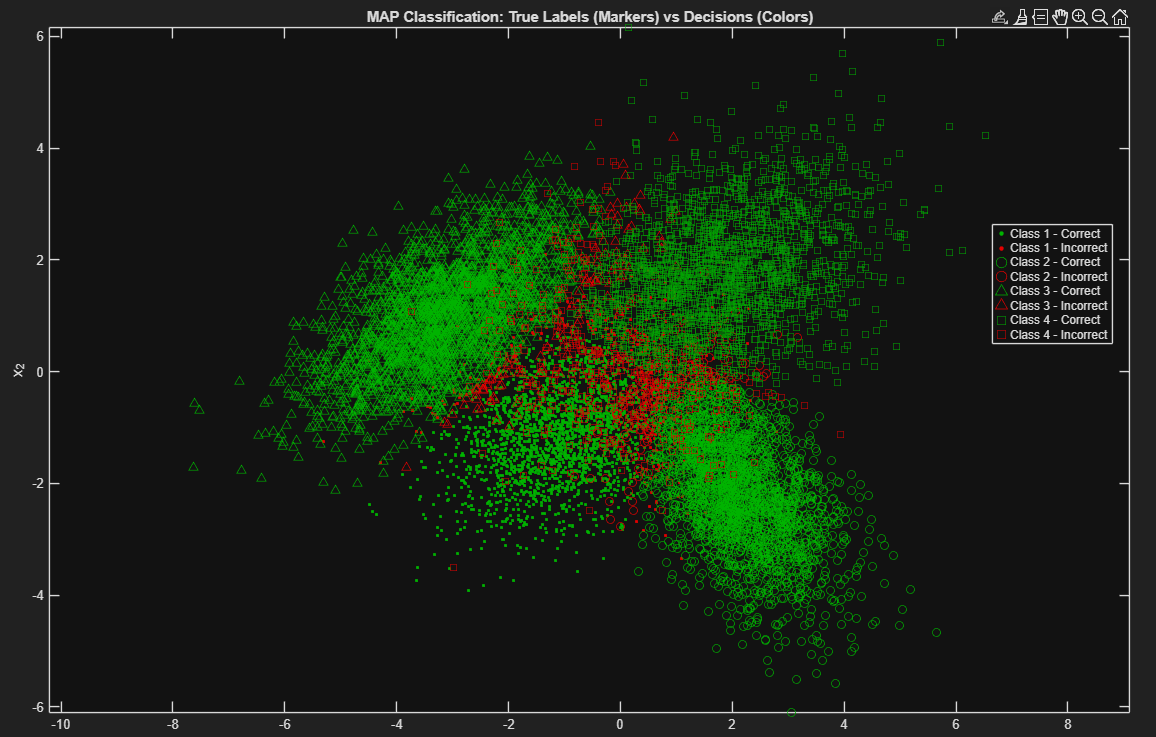
\includegraphics[width=0.7\textwidth]{map_classification.png}
\end{figure}

\subsubsection{Discussion}
The MAP classifier achieved 89.70\% overall accuracy with well-balanced performance across the four Gaussian classes. As expected, Class 4 demonstrated the lowest accuracy (83.93\%) due to its (intentionally) larger variance creating significant overlap with neighboring classes. The confusion matrix reveals that misclassifications primarily occurred between adjacent classes, with Class 4 samples being incorrectly assigned to Classes 1, 2, and 3 at rates of 8.79\%, 3.74\%, and 3.54\% respectively.

\subsection{Part B: ERM Classification with Asymmetric Loss}

\subsubsection{Theoretical Framework}
The ERM decision rule minimizes conditional risk:
\begin{equation}
\delta^*(\mathbf{x}) = \arg\min_{i \in \{1,2,3,4\}} R(D=i|\mathbf{x})
\end{equation}
where conditional risk is:
\begin{equation}
R(D=i|\mathbf{x}) = \sum_{j=1}^{4} \Lambda(i,j) P(L=j|\mathbf{x})
\end{equation}

The given loss matrix heavily penalizes Class 4 misclassification:
\[
\boldsymbol{\Lambda} = 
\begin{bmatrix}
0 & 10 & 10 & 100 \\
1 & 0 & 10 & 100 \\
1 & 1 & 0 & 100 \\
1 & 1 & 1 & 0
\end{bmatrix}
\]

\subsubsection{Implementation}
The ERM classifier computes posterior probabilities and selects decisions minimizing conditional risk.

\begin{figure}[H]
    \centering
    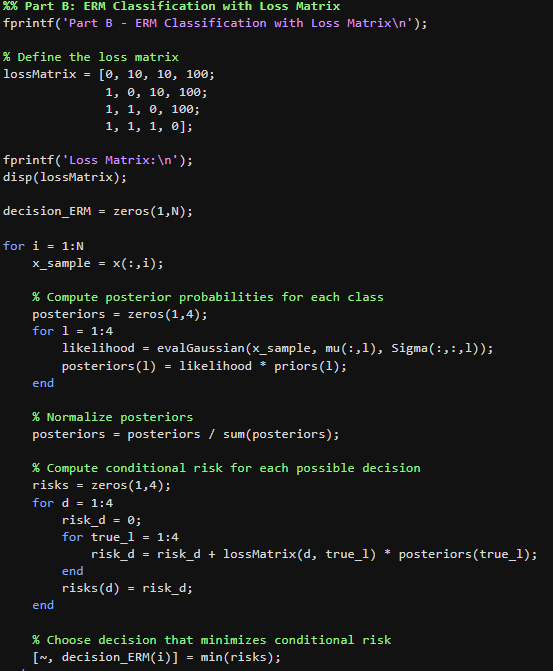
\includegraphics[width=0.6\textwidth]{q2_erm_code.png}
    \caption{ERM classification implementation}
\end{figure}

\subsubsection{Results}

\begin{figure}[H]
    \centering
    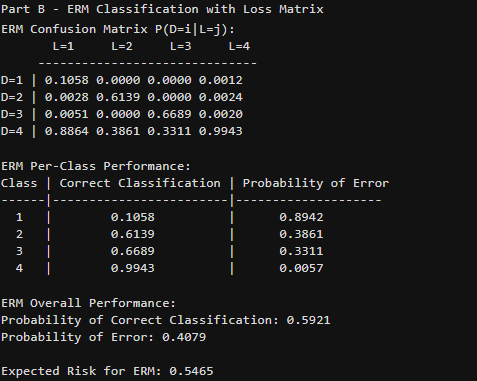
\includegraphics[width=0.6\textwidth]{q2_erm_output.png}
\end{figure}

\begin{figure}[H]
    \centering
    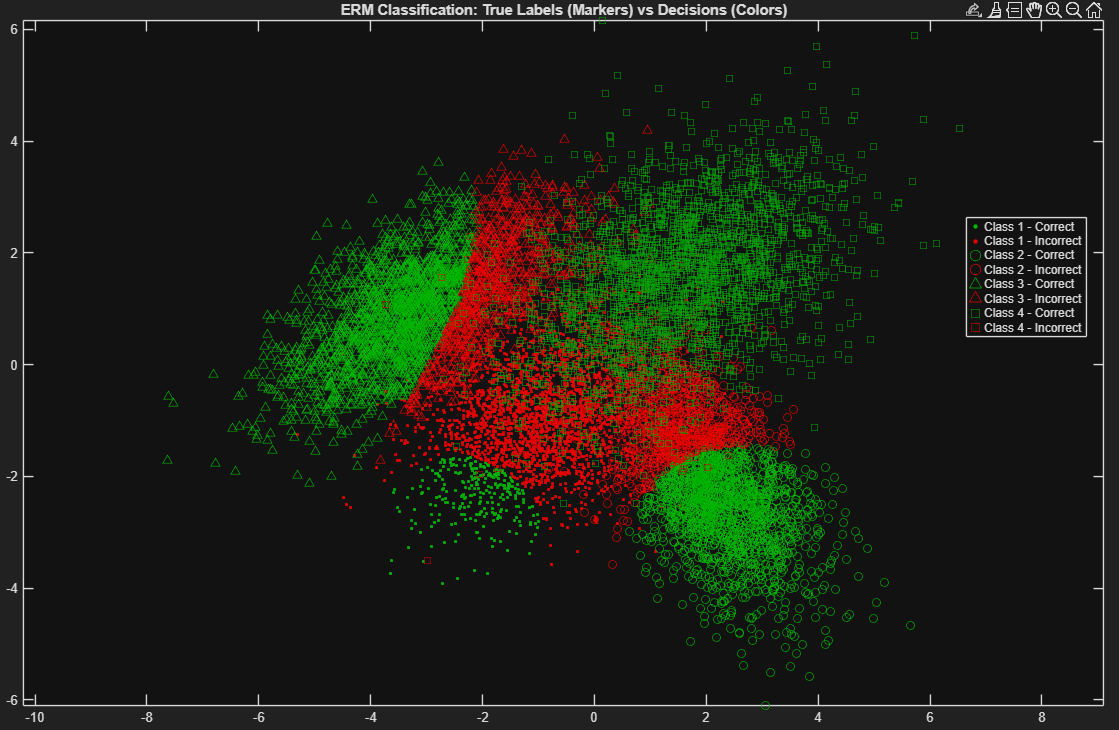
\includegraphics[width=0.8\textwidth]{erm_classification.png}
\end{figure}

\begin{figure}[H]
    \centering
    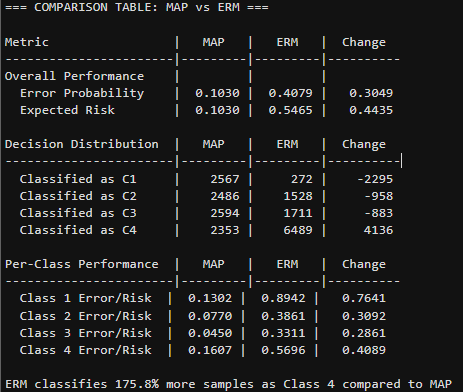
\includegraphics[width=0.6\textwidth]{q2_comparison_output.png}
\end{figure}

\subsubsection{Discussion}
The ERM classifier demonstrates how asymmetric loss structures reshape classification behavior. With a high penalty for Class 4 errors (loss = 100), the classifier becomes highly conservative, achieving 99.43\% Class 4 accuracy compared to 83.93\% with MAP. This protection comes at the cost of reduced performance for other classes, particularly Class 1 (86.98\% to 10.58\%). The classifier shows a 175.8\% increase in Class 4 assignments, and the expected risk of 0.5465 reflects the optimal balance under this cost structure, illustrating how decision boundaries adapt to error cost differentials.

% =============================================================================
% QUESTION 3
% =============================================================================

\newpage
\section{Question 3: Real Wolrd Data Classification with Gaussian Classifier}

\subsection{Problem Statement}
Implement minimum-probability-of-error classifiers for real-world datasets assuming Gaussian class-conditional distributions. For each class, estimate mean vectors and covariance matrices using sample averages, and class priors using sample counts. Apply regularization to handle ill-conditioned covariance matrices using $C_{\text{Regularized}} = C_{\text{SampleAverage}} + \lambda I$ where $\lambda = \alpha \cdot \frac{\text{trace}(C_{\text{SampleAverage}})}{\text{rank}(C_{\text{SampleAverage}})}$ with $0 < \alpha < 1$. Evaluate performance using confusion matrices and error probabilities, and analyze the appropriateness of Gaussian assumptions through data visualization and covariance analysis.

\subsection{Part A: Wine Quality Dataset Classification}

\subsubsection{Dataset Description}
The winequality-white.csv dataset consists of 4898 samples with 11  features and on the 12th column, with number from 3 to 9 indicating wine quality scores. The dataset exhibits significant class imbalance, with quality scores 5, 6, and 7 comprising 93.6\% of the data.

\subsubsection{Theoretical Framework}
The minimum-probability-of-error classification follows the MAP decision rule:

\begin{equation}
\delta^*(\mathbf{x}) = \arg\min_{j} \left[1 - P(L=j|\mathbf{x})\right] = \arg\max_{j} P(L=j|\mathbf{x})
\end{equation}
With Gaussian class-conditional distributions:
\begin{equation}
p(\mathbf{x}|L=j) = \frac{1}{(2\pi)^{11/2}|\boldsymbol{\Sigma}_j|^{1/2}} \exp\left(-\frac{1}{2}(\mathbf{x}-\boldsymbol{\mu}_j)^T\boldsymbol{\Sigma}_j^{-1}(\mathbf{x}-\boldsymbol{\mu}_j)\right)
\end{equation}

Regularization ensures numerical stability for ill-conditioned covariance matrices:
\begin{equation}
\boldsymbol{\Sigma}_j^{\text{reg}} = \boldsymbol{\Sigma}_j + \lambda\mathbf{I}, \quad \lambda = \alpha \cdot \frac{\text{trace}(\boldsymbol{\Sigma}_j)}{\text{rank}(\boldsymbol{\Sigma}_j)}
\end{equation}

\subsubsection{Implementation}
The Gaussian classifier was implemented in Python with feature standardization and covariance regularization.

\href{https://github.com/GuestAGuy/EECE5644/blob/main/HW1Q3/wine_dataset/gaussian_classifier.py}{https://github.com/GuestAGuy/EECE5644/blob/main/HW1Q3/wine_dataset/gaussian_classifier.py}

\begin{figure}[H]
    \centering
    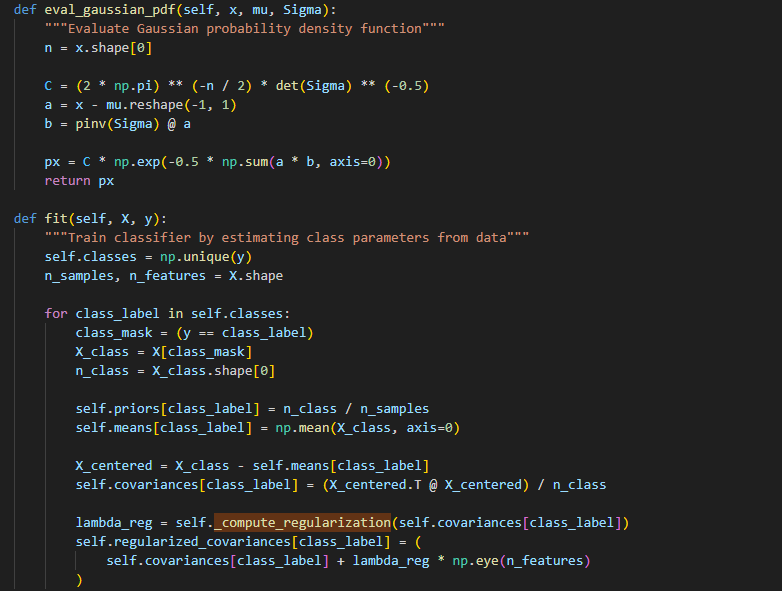
\includegraphics[width=0.8\textwidth]{gaussian_classifier_code.png}
    \caption{Gaussian classifier implementation with regularization}
\end{figure}

\begin{figure}[H]
    \centering
    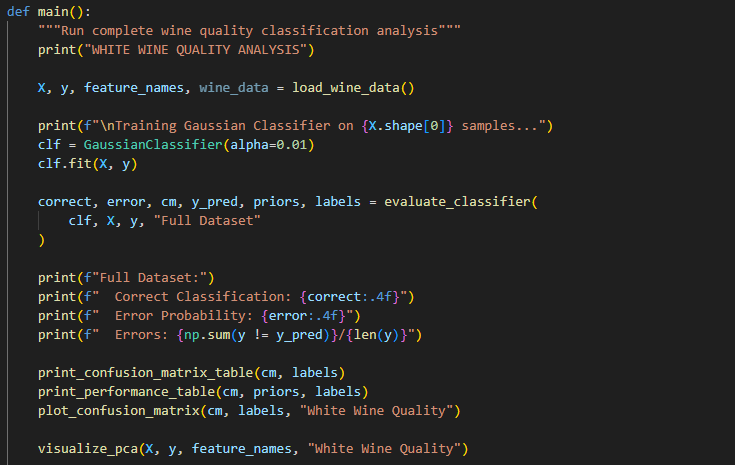
\includegraphics[width=0.8\textwidth]{wine_main_implementation.png}
    \caption{Wine quality classification implementation}
\end{figure}

\subsubsection{Results and Analysis}

\begin{figure}[H]
    \centering
    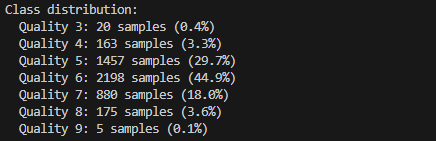
\includegraphics[width=0.6\textwidth]{wine_class_distribution.png}
\end{figure}

\begin{figure}[H]
    \centering
    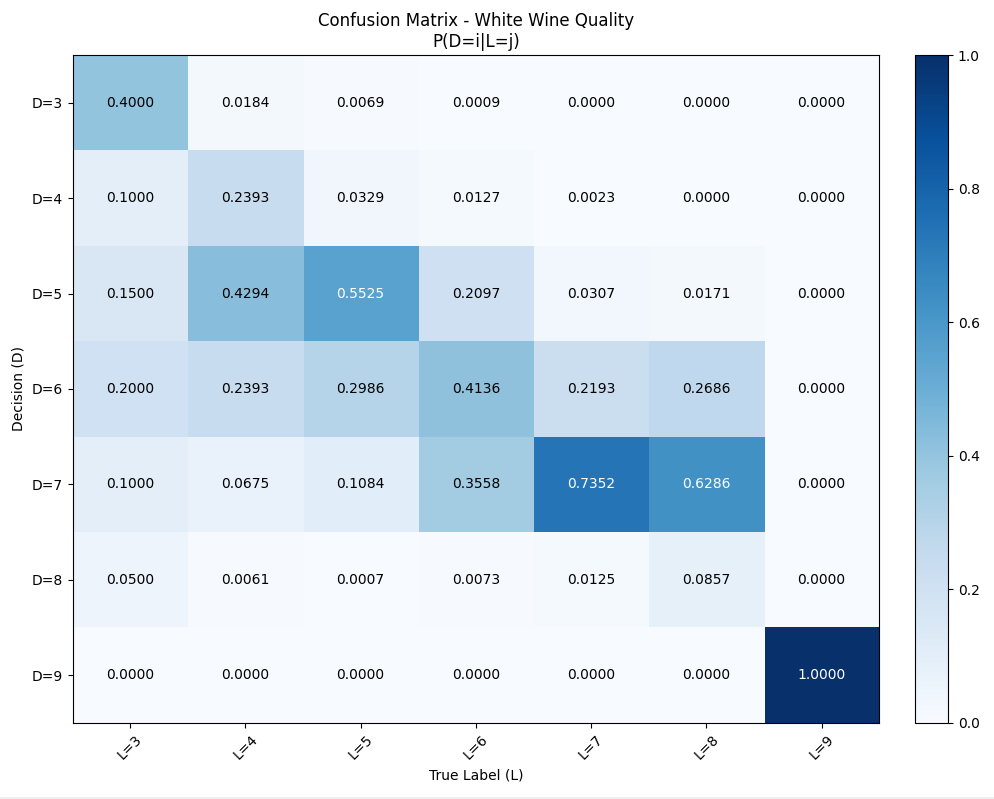
\includegraphics[width=0.8\textwidth]{wine_confusion_matrix_result.png}
\end{figure}

\begin{figure}[H]
    \centering
    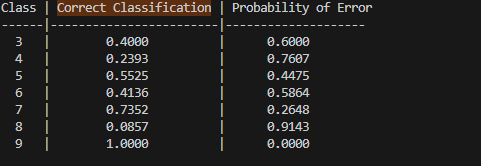
\includegraphics[width=0.6\textwidth]{wine_performance_result.png}
\end{figure}

\subsubsection{Data Visualization and Model Analysis}

\begin{figure}[H]
    \centering
    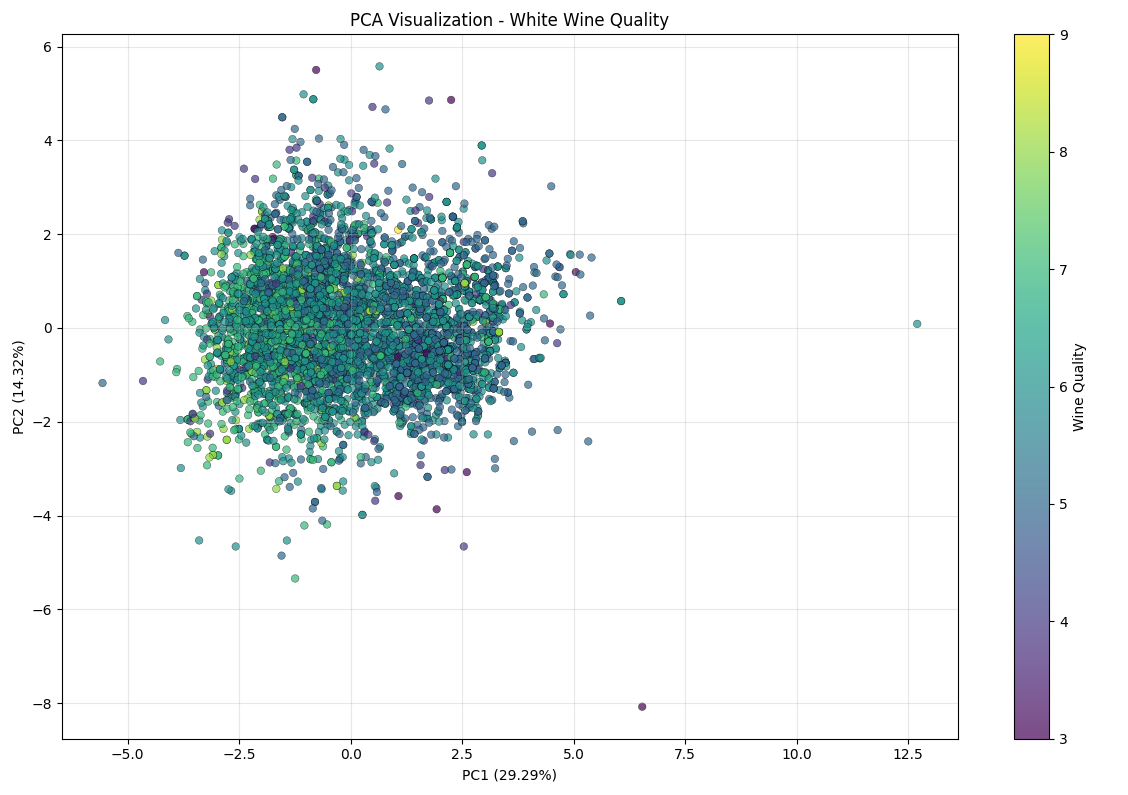
\includegraphics[width=0.8\textwidth]{wine_pca_analysis.png}
    \caption{PCA visualization and feature contribution analysis}
\end{figure}

\begin{figure}[H]
    \centering
    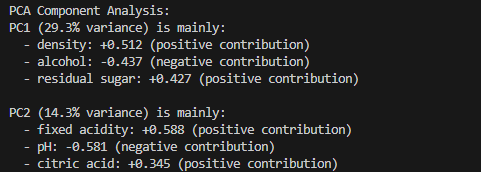
\includegraphics[width=0.6\textwidth]{wine_covariance_analysis.png}
    \caption{Covariance matrix condition number analysis across quality classes}
    \label{fig:wine_covariance_analysis}
\end{figure}

\subsubsection{Discussion}
The Gaussian classifier achieved 46.33\% correct classification on the wine quality dataset, revealing significant limitations in the Gaussian modeling assumption for this problem domain.

The fundamental issue lies in applying Gaussian distributions to data that likely follows more complex, non-Gaussian patterns. Wine quality assessment involves intricate relationships between physicochemical properties that cannot be adequately captured by simple elliptical Gaussian contours. The continuous nature of wine quality, evidenced by 85\% of misclassifications occurring between adjacent quality scores, suggests the underlying class-conditional distributions overlap in ways that Gaussian models cannot properly represent.

Severe class imbalance further exacerbates the model mismatch, with rare classes (3, 4, 8, 9 comprising only 7.4\% of data) having insufficient samples for meaningful Gaussian parameter estimation. The necessity of strong regularization, particularly for Class 9 where the condition number improved from $8.62\times10^{17}$ to $2.31\times10^{2}$, indicates fundamental instability in the Gaussian assumption rather than mere numerical issues.

While PCA revealed physically meaningful feature relationships (density, alcohol, and residual sugar as primary discriminators), the poor overall performance suggests these relationships are not well-modeled by Gaussian distributions. The suboptimal accuracy across most quality levels, particularly for intermediate scores 5 and 6 where classification should be most reliable, indicates systematic model mismatch rather than random error.

The results demonstrate that while the Gaussian classifier provides a mathematically tractable framework, its assumptions are inappropriate for the complex, continuous nature of wine quality assessment. The performance limitations stem from fundamental distributional mismatches that cannot be resolved through parameter tuning or regularization alone, suggesting alternative approaches capturing the continuous and potentially multi-modal nature of wine quality distributions would be more appropriate.

% =============================================================================
% PART B - PLACEHOLDER FOR HUMAN ACTIVITY DATASET
% =============================================================================

\subsection{Part B: Human Activity Recognition Dataset Classification}
 due to other homework, i decided to not do this part, for now
\subsubsection{Dataset Description}
[Human Activity dataset description placeholder]

\subsubsection{Implementation and Results}
[Human Activity implementation and results placeholder]

\subsubsection{Discussion}
[Human Activity discussion placeholder]

% =============================================================================
% COMPARATIVE ANALYSIS
% =============================================================================

\subsection{Comparative Analysis and Conclusions}

[Comparative analysis between Wine Quality and Human Activity datasets placeholder]

Key comparative aspects to analyze:
\begin{itemize}
\item Impact of feature dimensionality (11 vs 561 features)
\item Effects of class distribution characteristics
\item Regularization requirements across datasets
\item Gaussian assumption appropriateness in different domains
\item Performance limitations and error patterns
\end{itemize}
% =============================================================================
% CITATIONS
% =============================================================================

\newpage
\section*{Citations and External Assistance}

\subsection*{External Resources}
\begin{itemize}
    \item Course lectures, notes, code, for theoretical foundations of ERM classification, Naive Bayes, ROC curve, and Fisher LDA
    \item https://cs229.stanford.edu/section/cs229-gaussian_processes.pdf
    \item MATLAB documentation
    \item Python documentations
    \item Overleaf documentation for LaTeX typesetting
    \item https://www.geeksforgeeks.org/machine-learning/python-for-machine-learning/# for reviewing ML library in python
    \item Older jpynb I worked on 3 year ago
\end{itemize}

\subsection*{AI Assistance}
This assignment was completed with assistance from AI tools for:
\begin{itemize}
    \item Clarification and list of assignment requirements
    \item learning MATLAB
    \item Code structures, especially the on plotting and printing of data
    \item LaTeX document structure and mathematical typesetting in overleaf
    \item Theoretical concept verification and code debugging.
    \item Helping me going through question 3, list me many different way to possibly improve the accuracy, and let me understand the PCA.
\end{itemize}

All mathematical derivations, code implementation, analysis, and final conclusions are my own work or from "notes" and "code" provided in class. The AI assistance was used for reference when unsure how to code a certain structure(ie. plotting), use a certain library, clarification of concepts, and debugging.

\end{document}